%\subparagraph*{Inferring the Operational Space and Appropriate Controls with Multiple Contacts (T4.2)}

Within this task, IIT researched on a method for self calibrating the joint encoders offsets of a multibody system using inertial sensors measurements, then implemented and integrated this method in a sensor calibration and diagnosis application tool.\\

\textbf{Objective}\\

Accurate sensing of joint angles is a crucial requirement for effective dynamic whole-body control of humanoid robots. While, for standard robot platforms, some kinematic parametric models are typically extracted from the CAD diagrams, joint encoders offsets are assembly dependent. Therefore, the accurate calibration of such parameters is required after any repair task, and can be frequent. For that reason, a fast, accurate, automatic and in-situ method for calibrating joint encoders offsets was identified as a real necessity within the WP4 research scope. A method was proposed using multiple on-board inertial sensors. The method consists in aligning, for each accelerometer, the sensor measurements with the expected link acceleration vector expressed on the sensor frame. The computation of the expected link acceleration depends on the forward kinematics, including the joint offsets. The problem can then be posed as an over-constrained nonlinear least squares minimization process.\\

\textbf{Innovation}\\

Prior methods have been proposed in the same context: some use external kinematic constraints \cite{Hollerbach2008} \cite{Liu2009}; others use, as we do, inertial sensors and least-squares optimisation but focus on full kinematic parameters estimation, require specific recursive sequence of complex motion patterns, the accelerometers cross-axis sensitivity is not estimated and the calibration can only be performed joint by joint \cite{Wieser2011} \cite{Mittendorfer2012} \cite{Mittendorfer2014}. In contrast, the method we've proposed is novel in that: it doesn't require any external fixture or kinematic constraint, and thus is well suited for field deployments; the input data is acquired in a single slow motion and minimal sequence (we can assume that the measured acceleration is due only to gravity); the calibration is then done in a single optimization process for the complete set of joint encoders offsets; the accelerometers are fully calibrated in-situ within the same automated process (axis gains and cross-axis sensivity due to manufacturing tolerance); we take advantage of the a priori knowledge of the relative pose of each accelerometer with respect to its support link frame, extracted from the CAD diagrams. The calibration can also be done in a chain-wise fashion, independently for each limb.\\

\textbf{Implementation}\\

The minimization process is based on a cost function evaluating the gap between the measured and the expected gravity acceleration. The method was implemented on Matlab, using the Matlab Optimization Toolbox solver lsqnonlin along with the trust-region-reflective algorithm. The accelerometers  have been calibrated assuming that the sensor model is affine and using an ellipsoid fitting open source tool. Further more, a full diagnosis feature has been implemented for the cross validation of the computed calibration parameters. The tool is based on the same key performance indicators used for calibrating the sensors, and it plots: the distribution of the error on the measured accelerations magnitude; the time series and distribution of the angle between the measured and the expected accelerations; the fitting of the inertial sensor model to its manifold.\\

\textbf{Main Results}\\

The training data acquisition, the calibration procedure and the diagnosis/plotting tool have been integrated into a full Matlab application as a single script with a simplified user interface, suited for production teams or researchers using the iCub platform. The application has been validated on Gazebo simulation by using virtual ground truth joint encoders. For that purpose, we implemented a Gazebo-Yarp plugin emulating the iCub skin accelerometers measurements on the yarp interface. the application estimated the joint offsets from the inertial measurements with an accuracy of 0.005 degrees.

The application was tested on an iCub v2.5 fully equiped with the skin inertial sensors. The legs, torso and head inertial sensors and joint encoders were successfuly calibrated. The computed joint offsets were compared against the offsets measured manually, showing a gap always below 2 degrees. Furthermore, the angle error between the measured and the estimated gravity vector across all the inertial sensors is within 3 degrees, as we can see in figure \ref{fig:T4.2-selfCalibration-Diagnosis}, this error has been overall reduced by an average factor of 3. This performance should be improved in a future work by fine tuning the sensors orientation frames.

Furthermore, a formal analysis of the accuracy and observability will be performed in the next steps. The proposed method and initial results have been published as a paper \cite{GuedelhaSelfCalibJointOffsets2016} through the 2016 IEEE-RAS International Conference on Humanoid Robots. The application is being released on the github repository \url{https://github.com/robotology-playground/joint-offset-calib-inertial}.\\

\begin{figure}[hb!]
  \centering
    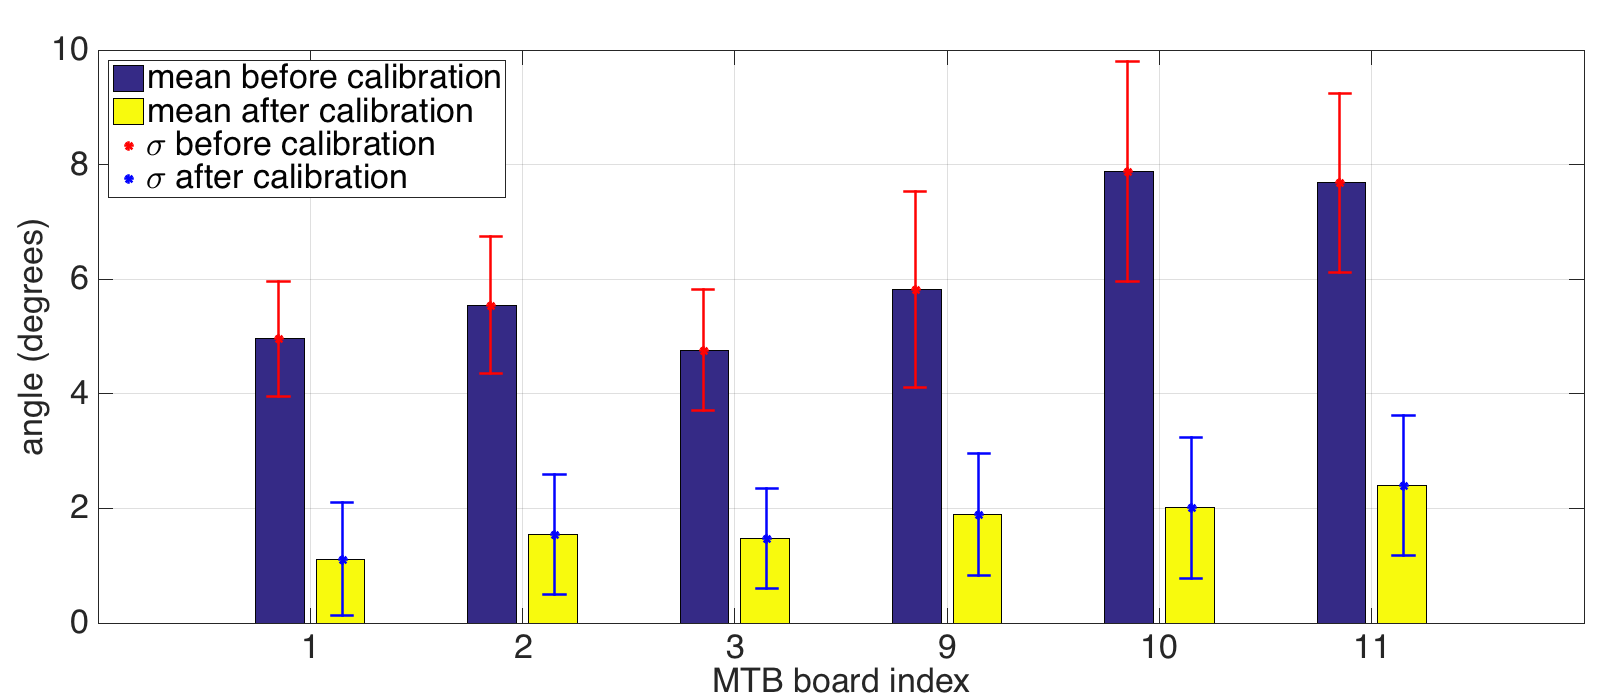
\includegraphics[width=0.8\textwidth]{images/T42-selfCalibration-Diagnosis.png}
    \caption{Diagnosis before and after calibration of the left leg joint encoders (angle of accelerometers measurements vs predictions)}
    \label{fig:T4.2-selfCalibration-Diagnosis}
\end{figure}
